\chapter{Dual and Reflexive spaces}

\section{Dual spaces}

\begin{fdefinition}
    Let $X$ be a normed space. The \textbf{dual space} of $X$, denoted by 
    $X^*$, is the set of all bounded linear functionals on $X$, i.e.:

    $$X^* = \Lcur(X, \R)$$

    It is a Banach space, with norm:

    $$\norm{L}_{X^*} = \norm{L}_* = \sup_{\norm{x}_X \leq 1} |Lx|$$
\end{fdefinition}

\begin{fexample}
    Let $X = L^p(\Omega, \M, \mu)$, with $1 \leq p \leq \infty$. Then,
    take the conjugate exponent $q$. Take $u \in L^q(\Omega, \M, \mu)$.
    Define $L_u \in (L^p(\Omega))^*$ as:

    $$L_u v = \int_{\Omega} uv \; d\mu \quad \forall v \in L^p(\Omega)$$

    Then, show that:
    \vspace{1em}
    \begin{enumerate}
        \item[0)] $L_u$ is well-defined:\\
        From Hölder's inequality, we have:

        $$|L_u v| = \left| \int_{\Omega} uv \; d\mu \right| \leq \norm{u}_q \norm{v}_p$$

        So $L_u v \in \R, \; \forall v \in L^p(\Omega)$. 
        \vspace{1em}

        \item[1)] $L_u$ is linear:
        $$L_u(\alpha_1 v_1 + \alpha_2 v_2) = \int_{\Omega} u(\alpha_1 v_1 + \alpha_2 v_2) \; d\mu =$$
        $$=\alpha_1 \int_{\Omega} u v_1 \; d\mu + \alpha_2 \int_{\Omega} u v_2 \; d\mu = \alpha_1 L_u v_1 + \alpha_2 L_u v_2$$
        \vspace{1em}

        \item[2)] $L_u$ is continuous:\\
        By Hölder's inequality, we also have that $\norm{L_u}_* \leq \norm{u}_q$.
        Then, $L_u$ is bounded, so it is continuous.
        \vspace{1em}

        \item[3)] Calculate $\norm{L_u}_*$:\\
        Assume that $p \in (1, \infty)$. Then:

        $$\norm{L_u}_* = \sup_{v \neq 0} \frac{|L_u v|}{\norm{v}_p} \geq \frac{|L_u \bar{v}|}{\norm{\bar{v}}_p} \quad \text{ for any } \bar{v} \neq 0$$

        Then we choose a $\bar{v}$ is such a way that $u \bar{v} = |u|^q$.

        $$\bar{v} = |u|^{\frac{q}{p}} \cdot sign(u)$$

        Notice that $u \in L^q \implies \bar{v} \in L^p$. Then:

        $$\norm{L_u}_* \geq \frac{|L_u v|}{\norm{v}_p} = \frac{\int_{\Omega} |u|^q \; d\mu}{\left( \int_{\Omega} |u|^q \; d\mu \right)^{\frac{1}{p}}}$$
        $$= \frac{\norm{u}_q^q}{\norm{u}_q} = \norm{u}_q^{\frac{q}{p}} = \norm{u}_q$$

        So $\norm{L_u}_* = \norm{u}_q$.
    \end{enumerate}

    \vspace{1em}

    \textbf{Question:} Are all elements of $(L^p)^*$ of the form $L_u$ for 
    some $u \in L^q$?\\

    \textbf{Answer:} Yes, for $p \in (1, \infty)$. This is known as the
    \textbf{Riesz representation theorem}, we will see 
    it later in the course.

\end{fexample}


\begin{fremark}
    The cases $p=1$ and $p = \infty$ are more delicate. In any case:

    $$p=\infty \implies \norm{L_u}_{(L^{\infty})^*} = \norm{u}_1$$
    
    $$p = 1, X \text{ is $\sigma$-finite} \implies \norm{L_u}_{(L^1)^*} = \norm{u}_{\infty}$$
\end{fremark}

\section{Hahn-Banach theorem and consequences}

\begin{ftheorem}[Hahn-Banach continuous extension theorem]
    Let $X$ be a normed space, $Y \subset X$ a subspace, and $L \in Y^*$.
    Then there exists $\tilde{L} \in X^*$ such that:

    $$\tilde{L} y = Ly \quad \forall y \in Y$$

    and $\norm{\tilde{L}}_{X^*} = \norm{L}_{Y^*}$.

\end{ftheorem}

\begin{proof}
    Omitted, based on the axiom of choice.

\end{proof}

\subsection{Consequences of H-B}

\begin{fcorollary}
    Let $X$ be a normed space, $x_0 \in X \setminus \{0\}$. Then 
    $\exists L \in X^*$ s.t.
    
    $$\norm{L}_{X^*} = 1, \quad L x_0 = \norm{x_0}_X$$

\end{fcorollary}

\begin{proof}
    Take $Y = span \{x_0\} = \{t x_0 : t \in \R\}$, and $L_0(t x_0) = t \norm{x_0}_X$.
    Notice that:
    \begin{enumerate}
        \item $L_0$ is well-defined, linear, and continuous.
        \item 
        $$\norm{L_0}_{Y^*} = \sup_{y \in Y, y \neq 0} \frac{|L_0 y|}{\norm{y}} = \sup_{t \neq 0} \frac{|L_0(tx_0)|}{\norm{tx_0}} = \sup_{t \neq 0} \frac{|t \norm{x_0}_X|}{|t| \norm{x_0}_X} = 1$$
    \end{enumerate}

    Then, by H-B, $\exists L \in X^*$ such that $L x_0 = \norm{x_0}_X$ and $\norm{L}_{X^*} = 1$.
\end{proof}

\begin{fcorollary}[Bounded linear functions separate points]
    $\forall x,y \in X$, normed space, we have:
    $$x \neq y \implies \exists L \in X^*: Lx \neq Ly$$

    I.e.:

    $$Lx = Ly \quad \forall L \in X^* \implies x = y$$
    
\end{fcorollary}

\begin{proof}
    Take $x \neq y$ and apply previous corollary to $x_0 = x - y \neq 0$. Then,
    $\exists L \in X^*$ such that $L(x-y) = \norm{x-y}_X \neq 0$, i.e., $Lx \neq Ly$.
\end{proof}

\begin{fcorollary}[Bounded linear functionals separate closed subspaces and points]
    Let $X$ be a normed space, $Y \subsetneq X$ a closed subspace,
    $x_0 \in X \setminus Y$. Then, $\exists L \in X^*$ such that: 

    $$Ly = 0, \quad \forall y \in Y \quad \text{ and } \quad Lx_0 \neq 0$$
    
\end{fcorollary}

\begin{proof}
    Take 
    $$Z = span \{x_0, Y\} = span \{x_0\} \oplus Y = \{z \in X: z = t x_0 + y, t \in \R, y \in Y\}$$

    Since $x_0 \notin Y$, for every $z \in Z$, $t, y$ are uniquely defined:

    $$t_1 x_0 + y_1 = t_2 x_0 + y_2$$ 
    $$\implies (t_1 - t_2) x_0 = y_1 - y_2$$ 

    and because $y_1 - y_2 \in Y$, but $x_0 \notin Y$, then $t_1 = t_2$ and $y_1 - y_2 = 0 \implies y_1 = y_2$.\\

    Let us define $L_0 : Z \to \R$ as $L_0(t x_0 + y) = t$. We have that
    $L_0 \in Z^*$, and:

    $$L_0 x_0 = L(1 \cdot x_0 + 0) = 1, \quad \text{ and } \quad L_0 y = L_0 (0 \cdot x_0 + y) = 0$$

    And we finally extend it to $L = \tilde{L_0}$ using H-B.

\end{proof}

\section{Reflexive spaces}

\begin{note}
    We have $X$ Banach, and $X^* = \Lcur(X, \R)$ Banach too. For notation, 
    we will use the following: $L \in X^{*}, x \in X$:

    $$L x = L(x) = \intprod{L}{x}$$

    And notice thar $\intprod{\cdot}{\cdot}$ is a \textbf{bilinear form}.
\end{note}

\begin{fdefinition}
    The bidual of $X$ is the dual of $X^*$, denoted by:

    $$X^{**} = (X^*)^* = \Lcur(X^*, \R)$$
\end{fdefinition}

\begin{fdefinition}
    Given $x \in X$ we can construct $\Lambda_x \in X^{**}$ as:
    $$\Lambda_x L = Lx \quad \forall L \in X^*$$

    Using the notation $\intprod{\cdot}{\cdot}$, we have:
    $$\intprod{\Lambda_x}{L} = \intprod{L}{x}$$

    The mapping $\tau: X \to X^{**}$ defined by $\tau(x) = \Lambda_x$ is called the
    \textbf{canonical map}.\\
\end{fdefinition}

\vspace{1em}

\begin{fproposition}
    $\forall x \in X$, $\Lambda_x \in X^{**}$, and
   the canonical map $\tau: X \to X^{**}$ is an isometry. In other words:

    $$\norm{\tau(x)}_{X^{**}} = \norm{x}_X \quad \forall x \in X$$

\end{fproposition}

\begin{proof}
    The proof goes as follows:
    \begin{itemize}
        \item \underline{$\Lambda_x$ is linear:} Indeed:
        $$\intprod{\Lambda_x}{L} = \intprod{L}{x}$$

        so it follows the linearity of $\intprod{\cdot}{x}$.

        \item \underline{$\Lambda_x$ is bounded:} It is implied by 
        \say{isometry}. Se below
    \end{itemize}

    \underline{Isometry:} We have that:

    $$\norm{\tau(x)}_{X^{**}} = \sup_{L \neq 0} \frac{|\intprod{\Lambda_x}{L}|}{\norm{L}_{X^*}} = \sup_{L \neq 0} \frac{|Lx|}{\norm{L}_{X^*}}$$

    Upper bounded:

    $$\sup_{L \neq 0} \frac{|Lx|}{\norm{L}_{X^*}} \leq \sup_{L \neq 0} \frac{\norm{L}_* \cdot \norm{x}}{\norm{L}_*} = \norm{x}$$

    Lower bounded:

    $$\sup_{L \neq 0} \frac{|Lx|}{\norm{L}_{X^*}} \geq \frac{|\bar{L} x|}{\norm{\bar{L}}_{X^*}} \quad \forall \bar{L} \neq 0$$

    By H-B, $\exists \tilde{L}$, s.t. $\tilde{L}x = \norm{x}$ and $\norm{\tilde{L}}_{X^*} = 1$. Then, if 
    $\bar{L} = \tilde{L}$, we have:

    $$\sup_{L \neq 0} \frac{|Lx|}{\norm{L}_{X^*}} \geq \frac{|\tilde{L} x|}{\norm{\tilde{L}}_{X^*}} = \norm{x}$$
\end{proof}

\begin{ftheorem}
    Let $\tau: X \to X^{**}$ be the canonical map. Then:
    \vspace{1em}
    \begin{itemize}
        \item it is linear and continuous.
        \vspace{1em}
        \item it is an isometry.
        \vspace{1em}
        \item it is injective.
        \vspace{1em}
        \item $R(\tau) \subset X^{**}$ is closed.
        \vspace{1em}
        \item it is a continuous embedding
    \end{itemize}
\end{ftheorem}

\begin{fremark}
    This means that we can think that $X$ is a closed subspace of $X^{**}$,
    i.e., $X \cong \tau(X)$, and $\tau(X) \subset X^{**}$ is a closed subspace.\\

    Notice that $\tau$ may be surjective, in which case $X \cong X^{**}$.
\end{fremark}

\vspace{1em}

\begin{fdefinition}
    We say that $X$ is \textbf{reflexive} if $\tau$ is surjective.
\end{fdefinition}

\vspace{1em}

\begin{note}
    To prove the previous theorem, we will use the following lemma:
\end{note}

\begin{flemma}[Nice properties of linear isometries]
    Take $X, Y$ Banach, $T: X \to Y$ linear such that:

    $$\norm{Tx}_Y = \norm{x}_X \quad \forall x \in X$$

    Then:
    \vspace{1em}
    \begin{enumerate}[label=(\roman*)]
        \item $T$ is continuous.
        \vspace{1em}
        \item $T$ is injective.
        \vspace{1em}
        \item $R(T) \subset Y$ is closed.
        \vspace{1em}
        \item $T: X \to R(T)$ is an isomorphism.
    \end{enumerate}
\end{flemma}

\begin{proof}
    The proof goes as follows:
    \begin{enumerate}[label=(\roman*)]
        \item $T$ linear $\implies$ $T$ continuous $\iff$ $T$ bounded. 
        Then, notice that:

        $$\norm{Tx}_Y \leq M \norm{x}_X \quad \forall x \in X$$

        is true for $M = 1$. Then, $T$ is continuous.

        \item Let $x, y \in X$ such that $Tx = Ty$. Then:
        $$T(x - y) = 0 \implies \norm{x-y}_X = 0 \implies x = y$$

        \item To show that $R(T)$ is closed, take $\{y_n\}_n \subset R(T)$ such that
        $y_n \to y \in Y$.  We want to show that $y \in R(T)$.\\

        Take $\{x_n\}_n$ such that $Tx_n = y_n$. Notice that
        since $\{y_n\}_n$ is Cauchy, and $\norm{y_n - y_m} = \norm{T(x_n - x_m)} = \norm{x_n - x_m}$,
        then $\{x_n\}_n$ is Cauchy too. Then, $\exists x \in X$ such that $x_n \to x$
        because $X$ is Banach. Now, since $T$ is continuous:

        $$Tx = T(\lim_{n \to \infty} x_n) = \lim_{n \to \infty} Tx_n = \lim_{n \to \infty} y_n = y$$

        Then, $y \in R(T)$.

        \item Since $T \in \Lcur(X, R(T))$ and $R(T)$ is closed (Banach), then
        $T$ is bijective between $X$ and $R(T)$. by a corollary of
        the open mappping theorem, $T^{-1}$ is continuous.
    \end{enumerate}
\end{proof}

\begin{proof}[Proof (theorem for $\tau$)]
    It is enough to check that:
    \begin{itemize}
        \item $\tau$ is linear (direct from linearity of $\intprod{\cdot}{\cdot})$
        \item $\tau$ is an isometry (already proved)
    \end{itemize}

\end{proof}

\subsection{Properties of reflexive spaces}

\begin{ftheorem}
    Let $X$ be Banach and reflexive. Let $Y \subset X$ closed subspace.
    Then, $Y$ is reflexive too.
\end{ftheorem}

\begin{ftheorem}
    Let $X$ be Banach. Then:
    $$X \text{ reflexive } \iff X \text{ reflexive }$$

\end{ftheorem}

\begin{ftheorem}
    Let $X$ be Banach. Then we have:
    $$X^* \text{ separable } \implies X \text{ separable }$$

    $$X \text{ reflexive and separable } \implies X^* \text{ reflexive and separable}$$
\end{ftheorem}

\begin{note}
    To check reflexivity, it is convenient to introduce the notion 
    of \textbf{uniformly convex space}
\end{note}

\vspace{1em}

\begin{fdefinition}
    We say that $X$ Banach is \textbf{uniformly convex} if $\forall \varepsilon > 0,
    \exists \delta > 0$ s.t.:

    $$\begin{cases}
        x, y \in X\\
        \norm{x} \leq 1, \norm{y} \leq 1\\
        \norm{x-y} > \varepsilon
    \end{cases} \implies \norm{\frac{x+y}{2} < 1 - \delta}$$
\end{fdefinition}

\begin{note}
    This is a \say{quantitative version} of the strict convexity of 
    $\overline{B_1(0)}$. In $\R^2$, is $\overline{B_1(0)}$ strictly convex?

    \begin{center}
        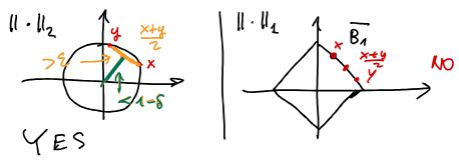
\includegraphics[width=0.8\textwidth]{figures/strict_convex.png}
    \end{center}

    One can see that, in $(\R^N, \norm{\cdot}_p)$, the property is true if and
    only if $p \in (1, \infty)$, and fails for $p = 1, \infty$.
\end{note}

\begin{ftheorem}[Millman-Pettis]
    $X$ Banach and uniformly convex $\implies X$ reflexive.
\end{ftheorem}

\begin{proof}
    Omitted. (Very difficult)
\end{proof}

\begin{fcorollary}
    $L^p(X)$ is reflexive for $p \in (1, \infty)$
\end{fcorollary}

\begin{fremark}
    $L^1(X)$ and $L^{\infty}(X)$ are \textbf{not} reflexive.
\end{fremark}

\section{Dual space of $L^p$}

\begin{ftheorem}[Riesz representation theorem (for $(L^p)^*$)]
    Let $(X, \M, \mu)$ be a complete measure space, $p \in (1, \infty)$,
    $q$ the conjugate exponent. Then:\\
    $\forall L \in (L^p(X))^*, \exists ! u \in L^q(X)$ s.t.:
    
    $$L v = \int_X uv \; d \mu, \quad \forall v \in L^p(X)$$

    Moreover, $\norm{L}_{(L^p)^*} = \norm{u}_{L^q}$.

\end{ftheorem}

\begin{fremark}
    We have already seen that $\forall u \in L^q(X)$, $L_u$ defined as:

    $$L_u v = \int_X uv \; d\mu$$

    is an element of $(L^p)^*$ and $\norm{L_u}_{(L^p)^*} = \norm{u}_{L^q}$.\\

    Moreover, for $T: L^q \to (L^p)^*$ s.t. $T(u) = L_u$, we obtain that 
    $T$ is an isometric isomorphism.
\end{fremark}

\begin{proof}
    By the \say{properties of isometries} and the example of last time,
    the only thing left to prove is that $T$ is surjective. This follows by H-B.

\end{proof}

\begin{ftheorem}
    For $p = 1$, $X$ $\sigma$-finite, we have that the $T: L^{\infty} \to (L^1)^*$ defined
    as:

    $$T(u) v = \int_X uv \; d\mu \forall v \in L^1$$

    is an isometric isomorphism, i.e., $(L^1)^* \cong L^{\infty}$.
\end{ftheorem}

\begin{ftheorem}
    For $p = \infty$, we have that $L^1 \hookrightarrow (L^{\infty})^*$, but the
    embedding is not surjective.
\end{ftheorem}

\vspace{1em}

\begin{fexample}
    We have that $\forall u \in L^1$, $L_u \in (L^{\infty})^*$, but
    $(L^{\infty})^*$ contains elements that are not of the form $L_u$.\\

    Take $L^{\infty}([-1, 1])$ and $C([-1, 1]) \subset L^{\infty}([-1, 1])$ 
    subspace. Then, take $L_0: C([-1, 1]) \to \R$ defined as:

    $$L_0 f = f(0)$$

    Then, $L_0$ is linear and bounded, so $L_0 \in (C([-1, 1]))^*$.\\

    By H-B, $\exists \tilde{L_0} \in (L^{\infty}([-1, 1]))^*$ such that

    $$\tilde{L_0} f = L_0 f \quad \forall f \in C([-1, 1]), \quad \norm{\tilde{L_0}}_{(L^{\infty})^*} = \norm{L_0}_{(C)^*}$$

    \textbf{Claim:} $\nexists u \in L^1([-1, 1])$ s.t. $\tilde{L_0} = L_u$.\\

    To show it, by contradiction, assume that $\exists u \in L^1$ s.t:

    $$\int_{-1}^1 u w \; d \mu = \tilde{L_0} w \quad w \in L^{\infty}$$

    Take $w_n$ s.t.:

    $$w_n = \begin{cases}
        1 - n |x| & |x| < \frac{1}{n}\\
        0 & \text{ otherwise}
    \end{cases}$$

    We can show that:
    \vspace{1em}
    \begin{itemize}
        \item $w_n(x) \to 0$ a.e.
        \vspace{1em}
        \item $|w_n(x)| \leq 1$ a.e.
        \vspace{1em}
        \item $(w_n u)(x) \to 0$ a.e.
        \vspace{1em}
        \item $|w_n(x) u(x)| \leq |u(x)| \in L^1$
    \end{itemize}
    \vspace{1em}

    Then, by DCT:

    $$\int_{-1}^1 u w_n \; d \lambda \to 0 \quad \text{ as } n \to \infty$$

    But:

    $$\tilde{L_0} w_n = L_0 w_n = w_n(0) = 1$$

    which is a contradiction.

\end{fexample}

\begin{note}[Resuming]
    For $L^p(\Omega, \Lcur(\Omega), \lambda)$, $\Omega \in \Lcur(\R^N)$ (but
    also $\ell^p$):
    \begin{center}
        \begin{tabular}{c|c|c|c|c}
            \textbf{Space} & \textbf{Completeness} & \textbf{Separability} & \textbf{Reflexivity} & \textbf{Dual}\\ \midrule
            $L^p, p \in (1, \infty)$ & Yes & Yes & Yes & $L^q, \frac{1}{p} + \frac{1}{q} = 1$\\ \midrule
            $L^1$ & Yes & Yes & No & $L^{\infty}$ \\ \midrule
            $L^{\infty}$ & Yes & No & No & $\supsetneq L^1$ \\ \bottomrule 
        \end{tabular}
    \end{center}
\end{note}


